% !TEX program = xelatex
\documentclass[11pt,a4paper]{article}

% ── Packages ──────────────────────────────────────────────────────────
\usepackage{ctex}                % Chinese support (requires XeLaTeX/LuaLaTeX)
\usepackage{amsmath,amssymb,amsfonts}
\usepackage{amsthm}
\usepackage{bm}
\usepackage{algorithm}
\usepackage{algpseudocode}
\usepackage{graphicx}
\usepackage{hyperref}
\usepackage{xcolor}
\usepackage[margin=2.5cm]{geometry}
\usepackage{booktabs}
\usepackage{tikz}

\hypersetup{
    colorlinks=true,
    linkcolor=blue,
    urlcolor=cyan,
    citecolor=green!50!black,
}

% ── Theorem Environments ──────────────────────────────────────────────
\newtheorem{definition}{Definition}[section]
\newtheorem{theorem}{Theorem}[section]
\newtheorem{remark}{Remark}[section]
\theoremstyle{definition}
\newtheorem{example}{Example}[section]

% ── Custom Commands ───────────────────────────────────────────────────
\newcommand{\E}{\mathbb{E}}
\newcommand{\R}{\mathbb{R}}
\newcommand{\N}{\mathcal{N}}          % Gaussian distribution
\newcommand{\D}{\mathcal{D}}
\newcommand{\X}{\mathcal{X}}
\newcommand{\Unif}{\mathcal{U}}       % uniform distribution
\newcommand{\KL}{D_{\text{KL}}}

% Macros for DDPM/DDIM (reused from diffusion.tex)
\newcommand{\alphat}{\bar{\alpha}_t}
\newcommand{\btd}{\tilde{\beta}_t}

\title{\Huge Image Inversion in Diffusion Models\\[0.3cm]
       \large Prompt-to-Prompt、Pivotal Inversion \& DDIM Inversion —— 原理推导与理解}
\author{}
\date{2026年6月3日}

\begin{document}
\maketitle
\tableofcontents
\newpage

% ═══════════════════════════════════════════════════════════════════════
%  1.  INTRODUCTION
% ═══════════════════════════════════════════════════════════════════════
\section{Introduction to Image Inversion}

\subsection{什么是 Inversion？为什么需要它？}

扩散模型（Diffusion Models）如 DDPM、DDIM 已经证明了自己在图像生成领域的强大能力。然而，仅仅能够\textbf{随机生成}图像是不够的——在实际应用中，我们更希望能够对\textbf{真实图像}进行编辑。

对于随机生成的图像，编辑相对简单：
\begin{itemize}
    \item 固定随机种子 $\Rightarrow$ 得到该图像来源的 latent code $z_T$ 和生成过程中的所有 feature
    \item 修改这些中间表示 $\Rightarrow$ 实现对生成图像的编辑
\end{itemize}

但对于\textbf{真实图像}（比如你手机里拍的照片），情况就完全不同了：
\begin{itemize}
    \item 我们没有它的 latent code $z_T$（不知道它对应什么噪声）
    \item 我们不知道它在生成过程中经过了哪些中间状态
    \item 无法直接套用随机生成图像的编辑方法
\end{itemize}

\textbf{Inversion（反演）的核心任务}就是：\textbf{给定一张真实图像，找到它在生成模型的 latent space 中对应的编码 $z_T$}，使得将这个编码送入冻结的生成器后，能够精准地重建出原图。

一旦成功反演，我们就可以：
\begin{enumerate}
    \item 在 latent space 中对 $z_T$ 进行操作
    \item 利用 cross-attention 等机制对中间特征进行调控
    \item 实现图像编辑（如局部修改、风格迁移、对象替换等）
\end{enumerate}

\subsection{Inversion 的核心挑战}

Inversion 任务的难点可以概括为一个两难困境（trade-off）：

\begin{center}
\begin{tabular}{c|c}
    \toprule
    \textbf{目标} & \textbf{挑战} \\
    \midrule
    重建保真度 (Reconstruction Fidelity) & 反演后的 $z_T$ 重建出的图像要尽可能接近原图 \\
    可编辑性 (Editability) & 反演得到的 latent code 要能支持有意义的编辑操作 \\
    \bottomrule
\end{tabular}
\end{center}

\textbf{为什么会存在这个 trade-off？} 直观理解：
\begin{itemize}
    \item 如果过分追求\textbf{重建精度}，$z_T$ 可能会"记住"原图的所有细节，但这些细节编码方式可能不是模型能理解的语义形式，导致编辑时牵一发而动全身。
    \item 如果过分追求\textbf{可编辑性}，$z_T$ 可能落在模型更容易操作的区域，但重建出来的图可能和原图有明显差异。
\end{itemize}

\textbf{个人理解：}这个 trade-off 本质上是"记忆 vs 理解"的矛盾。就像你背一篇课文——逐字背诵（完美重建）不一定代表你理解了内容（可编辑）。Inversion 要做的就是在"背下来"和"真懂"之间找到平衡点。

\subsection{Inversion 方法概览}

目前主流的 Inversion 方法可以分为几类：

\begin{center}
\begin{tabular}{c|c|c|c}
    \toprule
    \textbf{方法} & \textbf{核心思路} & \textbf{是否需要训练} & \textbf{编辑方式} \\
    \midrule
    DDIM Inversion & ODE 逆向求解 & 否 & latent space 操作 \\
    Pivotal Inversion & 直接优化 latent code & 否（优化 $z$） & cross-attention 调控 \\
    Prompt-to-Prompt & 修改 attention map & 否 & attention 替换/重加权 \\
    Textual Inversion & 学习新 token 的 embedding & 是（少量） & 新 token 触发 \\
    \bottomrule
\end{tabular}
\end{center}

本文将重点介绍\textbf{Prompt-to-Prompt}、\textbf{Pivotal Inversion} 和 \textbf{DDIM Inversion} 三种方法。


% ═══════════════════════════════════════════════════════════════════════
%  2.  PROMPT-TO-PROMPT
% ═══════════════════════════════════════════════════════════════════════
\section{Prompt-to-Prompt: 基于 Attention 的图像编辑}

\subsection{核心思想}

Prompt-to-Prompt（P2P）的思路出人意料地简单，但效果却非常好：

\begin{center}
\fbox{\textbf{文本提示词和生成图片的 attention map 有重要联系。}}
\end{center}

具体来说，在扩散模型的 U-Net 去噪过程中，cross-attention 层将文本 embedding 和图像特征关联起来。这些 attention map 决定了：
\begin{itemize}
    \item \textbf{哪些像素}受\textbf{哪些词}的影响
    \item 不同词对应的空间区域分布
\end{itemize}

因此，当我们想要编辑图像时，\textbf{只需要修改目标对象的 attention map}，就可以保持生成图片的其他部分不变，而只更改我们想要变更的那一部分。

\begin{figure}[ht]
    \centering
    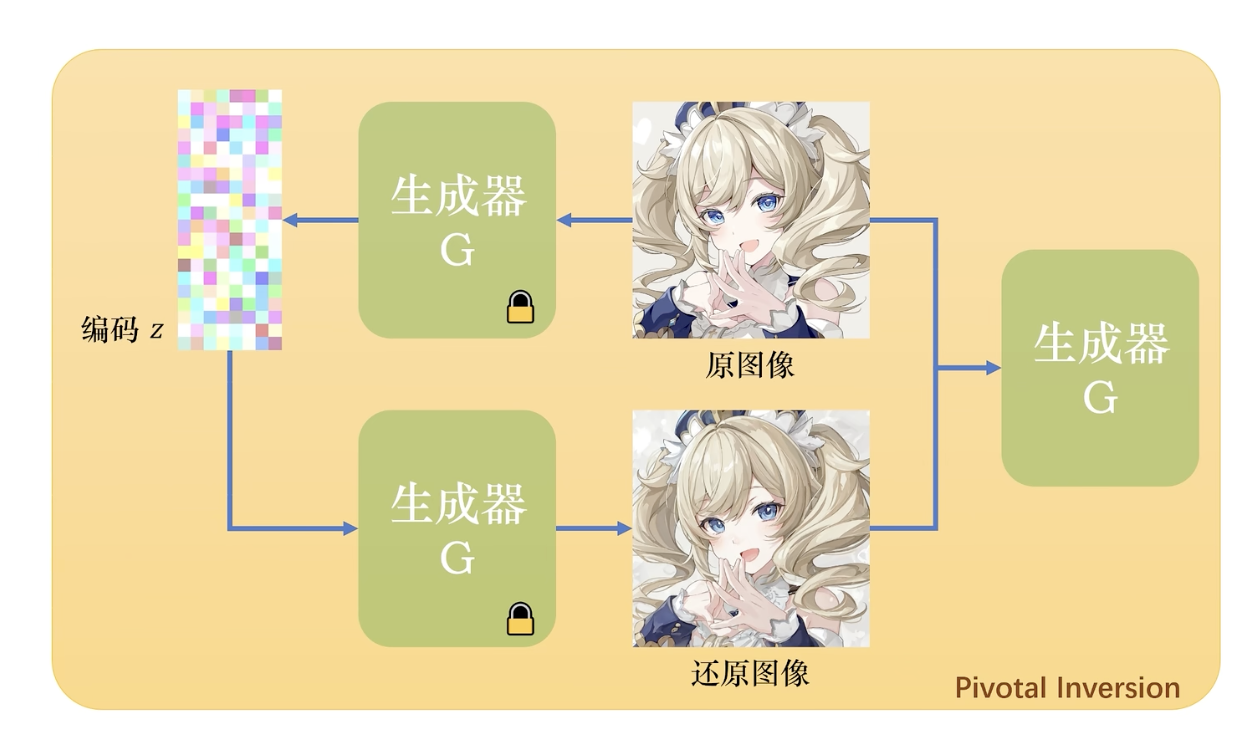
\includegraphics[width=0.85\textwidth]{images/image1.png}
    \caption{Prompt-to-Prompt 的核心直觉：通过替换/修改 attention map 来实现图像编辑，保持未编辑区域不变。}
    \label{fig:p2p_intuition}
\end{figure}

\subsection{Attention 机制回顾}

在扩散模型的 U-Net 中，cross-attention 层的计算方式为：

\begin{equation}\label{eq:cross_attention}
    \text{Attention}(Q, K, V) = \text{softmax}\!\left(\frac{Q K^T}{\sqrt{d}}\right) V
\end{equation}

其中：
\begin{itemize}
    \item $Q = W_Q \cdot \phi(x_t)$ —— 来自图像空间特征（spatial features）的 query
    \item $K = W_K \cdot \psi(P)$ —— 来自文本 prompt embedding 的 key
    \item $V = W_V \cdot \psi(P)$ —— 来自文本 prompt embedding 的 value
    \item $\phi(x_t)$ 是 U-Net 中间层的 spatial feature map
    \item $\psi(P)$ 是文本 prompt $P$ 经过 CLIP text encoder 得到的 embedding
\end{itemize}

Attention map $M_t$ 记录了在时间步 $t$、每个空间位置对每个文本 token 的"关注程度"：

\begin{equation}\label{eq:attention_map}
    M_t = \text{softmax}\!\left(\frac{Q K^T}{\sqrt{d}}\right)
\end{equation}

$M_t$ 的维度为 $(\text{spatial tokens}) \times (\text{text tokens})$——每个元素 $M_t[i, j]$ 表示第 $i$ 个空间位置对第 $j$ 个文本 token 的注意力权重。

\subsection{三种编辑操作}

Prompt-to-Prompt 提出了三种基于 attention map 操作的编辑方式：

\subsubsection{Word Swap（词替换）}

将源 prompt 中的某个词替换为目标 prompt 中的新词，同时将原词对应的 attention map 替换为新词的 attention map。

\textbf{例子：}将 "a photo of a \textbf{cat}" 改为 "a photo of a \textbf{dog}"，把 "cat" 对应的 attention 换为 "dog" 的 attention。

\subsubsection{Adding a New Phrase（添加新短语）}

在原 prompt 基础上添加修饰词，使用原图的 attention map 来保持未修改部分不变，只让新词影响其对应的区域。

\textbf{例子：}将 "a photo of a car" 改为 "a photo of a \textbf{red} car"，保持 "car" 区域的 attention 不变，让 "red" 的 attention 只影响车的颜色。

\subsubsection{Attention Re-weighting（注意力重加权）}

增加或减少某个词对应的 attention 权重，从而增强或减弱该词对生成图像的影响程度。

\textbf{例子：}让 "fluffy" 的 attention 权重翻倍，使生成的动物更加毛茸茸。

\subsection{算法流程}

\begin{algorithm}[ht]
\caption{Prompt-to-Prompt Editing}
\label{alg:p2p}
\begin{algorithmic}[1]
\Require 源图像 $x$，源 prompt $P$，目标 prompt $P^*$，编辑类型
\Ensure 编辑后的图像 $x^*$
\State 用 DDIM Inversion 反演 $x$ 得到 noise sequence $\{z_t\}$
\State 从 $z_T$ 开始逆向去噪
\For{$t = T, T-1, \dots, 1$}
    \State 用源 prompt $P$ 计算 attention maps $\{M_t\}$
    \If{编辑类型 = Word Swap}
        \State 用目标 prompt $P^*$ 重新计算 attention maps $\{M_t^*\}$
        \State 将指定 token 的 $M_t$ 替换为 $M_t^*$
    \ElsIf{编辑类型 = Adding Phrase}
        \State 用 $P^*$ 生成新的 attention，但固定原词对应的 attention 不变
    \ElsIf{编辑类型 = Re-weighting}
        \State $M_t[j] \leftarrow c \cdot M_t[j]$（对 token $j$ 重加权）
    \EndIf
    \State 用修改后的 attention map 进行去噪步骤
\EndFor
\State \Return $x^*$
\end{algorithmic}
\end{algorithm}

\textbf{注意：}Prompt-to-Prompt 的关键步骤是先用 DDIM Inversion 获取源图像的 noise sequence。这里就能看出 DDIM 确定性的重要性——如果逆向过程是随机的（如 DDPM），就没办法精确反演原图了。

\subsection{为什么有效？——直观理解}

可以把 cross-attention 理解为一个\textbf{布局分配器}：
\begin{itemize}
    \item 每个文本 token 通过 attention 来"认领"图像中的某些空间区域
    \item "猫"这个 token 会关注图像中猫所在的位置
    \item 如果我们把"猫"的 attention map 换成"狗"的 attention map，其他区域不变，那么猫就会变成狗，而背景保持原样
\end{itemize}

这也是为什么 Prompt-to-Prompt 能够实现\textbf{局部编辑}——因为 attention map 天然地将编辑操作限定在了对应的空间区域内。


% ═══════════════════════════════════════════════════════════════════════
%  3.  PIVOTAL INVERSION
% ═══════════════════════════════════════════════════════════════════════
\section{Pivotal Inversion: 直接优化 Latent Code}

\subsection{核心思想}

与 DDIM Inversion 的"递推式逆向求解"不同，Pivotal Inversion 采用了一种更直接的方法：\textbf{优化}。

核心思路：
\begin{enumerate}
    \item 固定扩散生成器 $G$（预训练好的 DDPM/Stable Diffusion 模型），参数不更新
    \item 以输入原图 $x$ 为约束基准
    \item 迭代优化隐编码 $z$（优化变量就是 $z$ 本身）
    \item 将 $z$ 送入冻结的生成器 $G$ 重建出 $\hat{x} = G(z)$
    \item 不断缩小原图 $x$ 与重建图像 $\hat{x}$ 的像素损失
    \item 最终得到能够精准复原原图的隐变量 $z^*$
\end{enumerate}

\begin{figure}[ht]
    \centering
    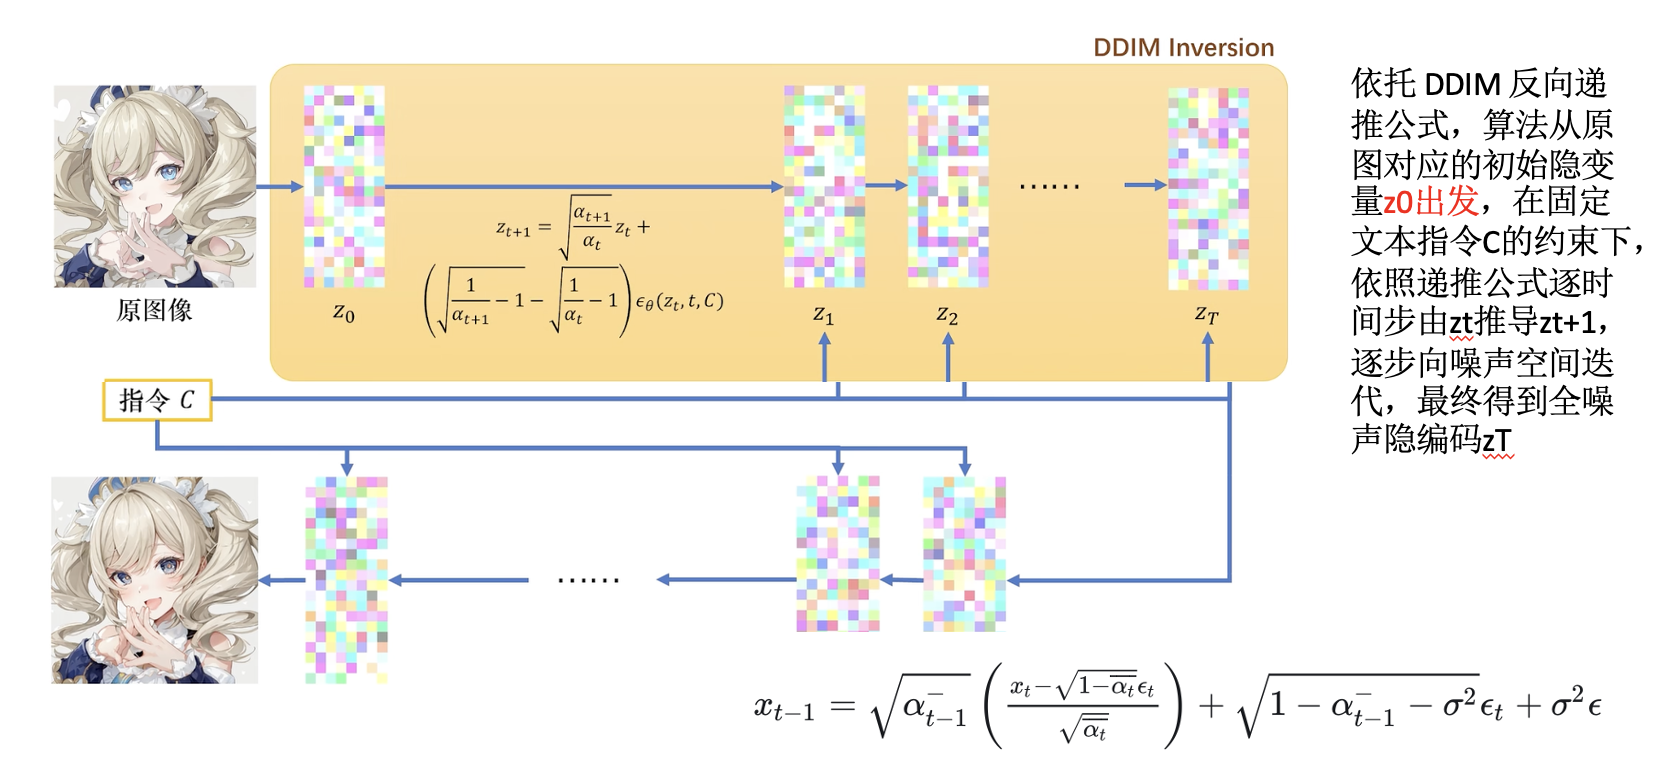
\includegraphics[width=0.85\textwidth]{images/image2.png}
    \caption{Pivotal Inversion 的优化流程：固定生成器 $G$，通过梯度下降直接优化 latent code $z$，使得 $G(z)$ 逼近原图 $x$。}
    \label{fig:pivotal_flow}
\end{figure}

\subsection{数学形式}

Pivotal Inversion 的优化目标可以形式化地写为：

\begin{equation}\label{eq:pivotal_objective}
    z^* = \arg\min_z \; \mathcal{L}\big(G(z),\, x\big)
\end{equation}

其中：
\begin{itemize}
    \item $z \in \R^d$ 是 latent code（通常是生成器的输入噪声或 StyleGAN 的 $\mathcal{W}^+$ 空间编码）
    \item $G(\cdot)$ 是冻结的生成器（权重不参与梯度更新）
    \item $x$ 是目标真实图像
    \item $\mathcal{L}$ 是损失函数
\end{itemize}

损失函数通常包含多个分量：

\begin{equation}\label{eq:pivotal_loss}
    \mathcal{L} = \lambda_{\text{pixel}} \mathcal{L}_{\text{pixel}} + \lambda_{\text{percept}} \mathcal{L}_{\text{percept}} + \lambda_{\text{reg}} \mathcal{L}_{\text{reg}}
\end{equation}

\subsubsection{Pixel Loss（像素损失）}

最基本的重建损失，逐像素比较：

\begin{equation}\label{eq:pixel_loss}
    \mathcal{L}_{\text{pixel}} = \| G(z) - x \|_2^2
\end{equation}

\subsubsection{Perceptual Loss（感知损失）}

仅用像素损失往往会导致重建图像模糊（因为逐像素 MSE 会倾向于平均化所有可能的解）。感知损失通过比较预训练网络（如 VGG）的中间特征层来保真：

\begin{equation}\label{eq:perceptual_loss}
    \mathcal{L}_{\text{percept}} = \sum_{l} \big\| \phi_l(G(z)) - \phi_l(x) \big\|_2^2
\end{equation}

其中 $\phi_l(\cdot)$ 是 VGG（或其他预训练网络）第 $l$ 层的特征图。

\subsubsection{Regularization（正则化）}

为了防止 $z$ 偏离模型的正常 latent 分布太远（导致编辑性下降），通常加入正则项：

\begin{equation}\label{eq:latent_reg}
    \mathcal{L}_{\text{reg}} = \| z - \mu_z \|_2^2
\end{equation}

或者限制 $z$ 在 latent space 的合理范围内（如在 $\mathcal{W}^+$ 空间中的截断）。

\subsection{优化过程}

\begin{algorithm}[ht]
\caption{Pivotal Inversion}
\label{alg:pivotal}
\begin{algorithmic}[1]
\Require 真实图像 $x$，冻结的生成器 $G$，学习率 $\eta$，迭代次数 $N$
\Ensure 最优 latent code $z^*$
\State 初始化 $z$（随机采样或使用 encoder 预测）
\For{$i = 1, \dots, N$}
    \State $\hat{x} = G(z)$ \Comment{前向传播，重建图像}
    \State $\mathcal{L} = \lambda_1 \|\hat{x} - x\|_2^2 + \lambda_2 \sum_l \|\phi_l(\hat{x}) - \phi_l(x)\|_2^2 + \lambda_3 \|z\|_2^2$
    \State $z \leftarrow z - \eta \cdot \nabla_z \mathcal{L}$ \Comment{只更新 $z$，不更新 $G$ 的参数}
\EndFor
\State \Return $z^* = z$
\end{algorithmic}
\end{algorithm}

\subsection{编辑：配合 Cross-Attention 调控}

得到 $z^*$ 后，就可以配合 cross-attention 调控实现原图的精细化局部编辑：

\begin{enumerate}
    \item 将 $z^*$ 送入生成器，同时记录每一层的 cross-attention maps
    \item 修改目标区域的 attention map（如替换、重加权、mask 等）
    \item 用修改后的 attention 重新生成，得到编辑后的图像
\end{enumerate}

\begin{figure}[ht]
    \centering
    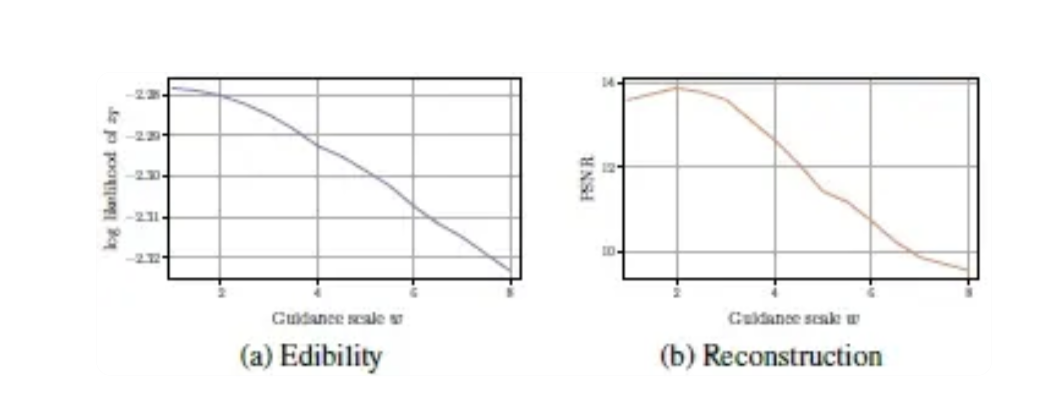
\includegraphics[width=0.85\textwidth]{images/image3.png}
    \caption{配合 cross-attention 调控的编辑流程：从反演得到的 $z^*$ 出发，在去噪过程中修改 attention maps，实现精细化的局部编辑。}
    \label{fig:pivotal_edit}
\end{figure}

\subsection{Pivotal Inversion vs DDIM Inversion}

\begin{center}
\begin{tabular}{c|c|c}
    \toprule
    \textbf{对比维度} & \textbf{Pivotal Inversion} & \textbf{DDIM Inversion} \\
    \midrule
    求解方式 & 直接优化 latent code $z$ & ODE 逆向递推 \\
    计算开销 & 需要多轮梯度迭代（较慢） & 类似正向采样的开销（较快） \\
    重建精度 & 通常更高（直接优化目标） & 取决于步数和 CFG scale \\
    对模型结构的依赖 & 只需要 $G$ 可微分 & 需要知道具体的采样器细节 \\
    latent 空间 & 可以在更灵活的 latent space 操作 & 限定在扩散模型的 noise space \\
    \bottomrule
\end{tabular}
\end{center}

\textbf{个人理解：}Pivotal Inversion 的"优化"思路比 DDIM Inversion 的"递推"思路更通用——前者只需要"生成器可微分"这一个条件，不关心内部是什么结构。但代价是慢，因为需要跑几十上百轮梯度下降。实际应用中，经常先用 DDIM Inversion 得到一个近似解，再用 Pivotal Inversion 做几步微调——把两者的优势结合起来。


% ═══════════════════════════════════════════════════════════════════════
%  4.  DDIM INVERSION
% ═══════════════════════════════════════════════════════════════════════
\section{DDIM Inversion: 基于 ODE 的逆向求解}

\subsection{回顾 DDIM 的确定性采样}

在之前的笔记（\texttt{diffusion.tex}）中，我们详细推导了 DDIM 的采样公式。回顾一下 DDIM 确定性采样（$\eta=0$）的核心公式：

正向一步（已知 $x_t$ 预测 $x_{t-1}$）：
\begin{equation}\label{eq:ddim_forward_rev}
    x_{t-1} = \sqrt{\bar{\alpha}_{t-1}}\, \hat{x}_0 + \sqrt{1 - \bar{\alpha}_{t-1}}\, \epsilon_\theta(x_t, t)
\end{equation}

其中 $\hat{x}_0$ 是对原图 $x_0$ 的预测：
\begin{equation}\label{eq:ddim_x0_hat}
    \hat{x}_0 = \frac{x_t - \sqrt{1 - \alphat}\, \epsilon_\theta(x_t, t)}{\sqrt{\alphat}}
\end{equation}

DDIM Inversion 的本质就是把上面的公式\textbf{倒过来用}——已知 $x_{t-1}$，求 $x_t$（即从干净图走向噪声）。

\subsection{DDIM Inversion 的推导}

在 DDIM 确定性采样的设定下，逆向过程（从 $x_t$ 到 $x_{t-1}$）是确定性的。因此我们可以直接对公式~(\ref{eq:ddim_forward_rev})进行代数变换，反解出 $x_t$：

将式~(\ref{eq:ddim_x0_hat})代入式~(\ref{eq:ddim_forward_rev})：

\begin{align}
    x_{t-1} &= \sqrt{\bar{\alpha}_{t-1}}\, \frac{x_t - \sqrt{1 - \alphat}\, \epsilon_\theta(x_t, t)}{\sqrt{\alphat}}
              + \sqrt{1 - \bar{\alpha}_{t-1}}\, \epsilon_\theta(x_t, t) \\[4pt]
            &= \frac{\sqrt{\bar{\alpha}_{t-1}}}{\sqrt{\alphat}}\, x_t
               - \frac{\sqrt{\bar{\alpha}_{t-1}}\sqrt{1 - \alphat}}{\sqrt{\alphat}}\, \epsilon_\theta(x_t, t)
               + \sqrt{1 - \bar{\alpha}_{t-1}}\, \epsilon_\theta(x_t, t) \\[4pt]
            &= \frac{\sqrt{\bar{\alpha}_{t-1}}}{\sqrt{\alphat}}\, x_t
               + \left(\sqrt{1 - \bar{\alpha}_{t-1}} - \frac{\sqrt{\bar{\alpha}_{t-1}}\sqrt{1 - \alphat}}{\sqrt{\alphat}}\right) \epsilon_\theta(x_t, t)
\end{align}

在\textbf{步长足够小}的假设下（即 $\alpha_t \approx 1$，$x_t \approx x_{t-1}$），我们可以近似 $\epsilon_\theta(x_t, t) \approx \epsilon_\theta(x_{t-1}, t)$。于是反解出 Inversion 的核心公式：

\begin{equation}\label{eq:ddim_inversion}
    x_t \approx \frac{\sqrt{\alphat}}{\sqrt{\bar{\alpha}_{t-1}}}\, x_{t-1}
            + \sqrt{\alphat}\left(\sqrt{\frac{1}{\alphat} - 1} - \sqrt{\frac{1}{\bar{\alpha}_{t-1}} - 1}\right) \epsilon_\theta(x_{t-1}, t)
\end{equation}

或者写作更对称的形式：
\begin{equation}\label{eq:ddim_inversion_v2}
    x_t = \sqrt{\frac{\alphat}{\bar{\alpha}_{t-1}}}\, x_{t-1}
        + \left(\sqrt{1 - \alphat} - \sqrt{\frac{\alphat(1 - \bar{\alpha}_{t-1})}{\bar{\alpha}_{t-1}}}\right) \epsilon_\theta(x_{t-1}, t)
\end{equation}

\textbf{直观理解：}DDIM Inversion 就是从 $x_0$（真实图像）出发，一步步往噪声方向走，用 U-Net 预测的噪声来"补充"每一步丢失的信息。走完 $T$ 步后得到 $x_T \approx z_T$，这个 $z_T$ 就是原图在 latent space 中的编码。

\subsection{Classifier-Free Guidance 下的 Inversion}

在实际使用中，扩散模型几乎都会配合 Classifier-Free Guidance (CFG) 来提升生成质量。CFG 的噪声预测公式为：

\begin{equation}\label{eq:cfg_noise}
    \tilde{\epsilon}_\theta(x_t, t, C) = \epsilon_\theta(x_t, t, \varnothing) + w \cdot \big(\epsilon_\theta(x_t, t, C) - \epsilon_\theta(x_t, t, \varnothing)\big)
\end{equation}

其中：
\begin{itemize}
    \item $C$ 是文本条件（text prompt）
    \item $\varnothing$ 是空文本（null text）
    \item $w$ 是 guidance scale，通常取 $w \in [1, 20]$，典型值为 $7.5$
\end{itemize}

\textbf{CFG 对 Inversion 的影响非常大：}

\begin{center}
\begin{tabular}{c|c|c}
    \toprule
    \textbf{$w$ 的取值} & \textbf{重建质量} & \textbf{可编辑性} \\
    \midrule
    $w$ 小（如 $w=1$） & 高（几乎完美重建） & 高 \\
    $w$ 大（如 $w=7.5$） & 低（有明显偏差） & 低 \\
    \bottomrule
\end{tabular}
\end{center}

\begin{figure}[ht]
    \centering
    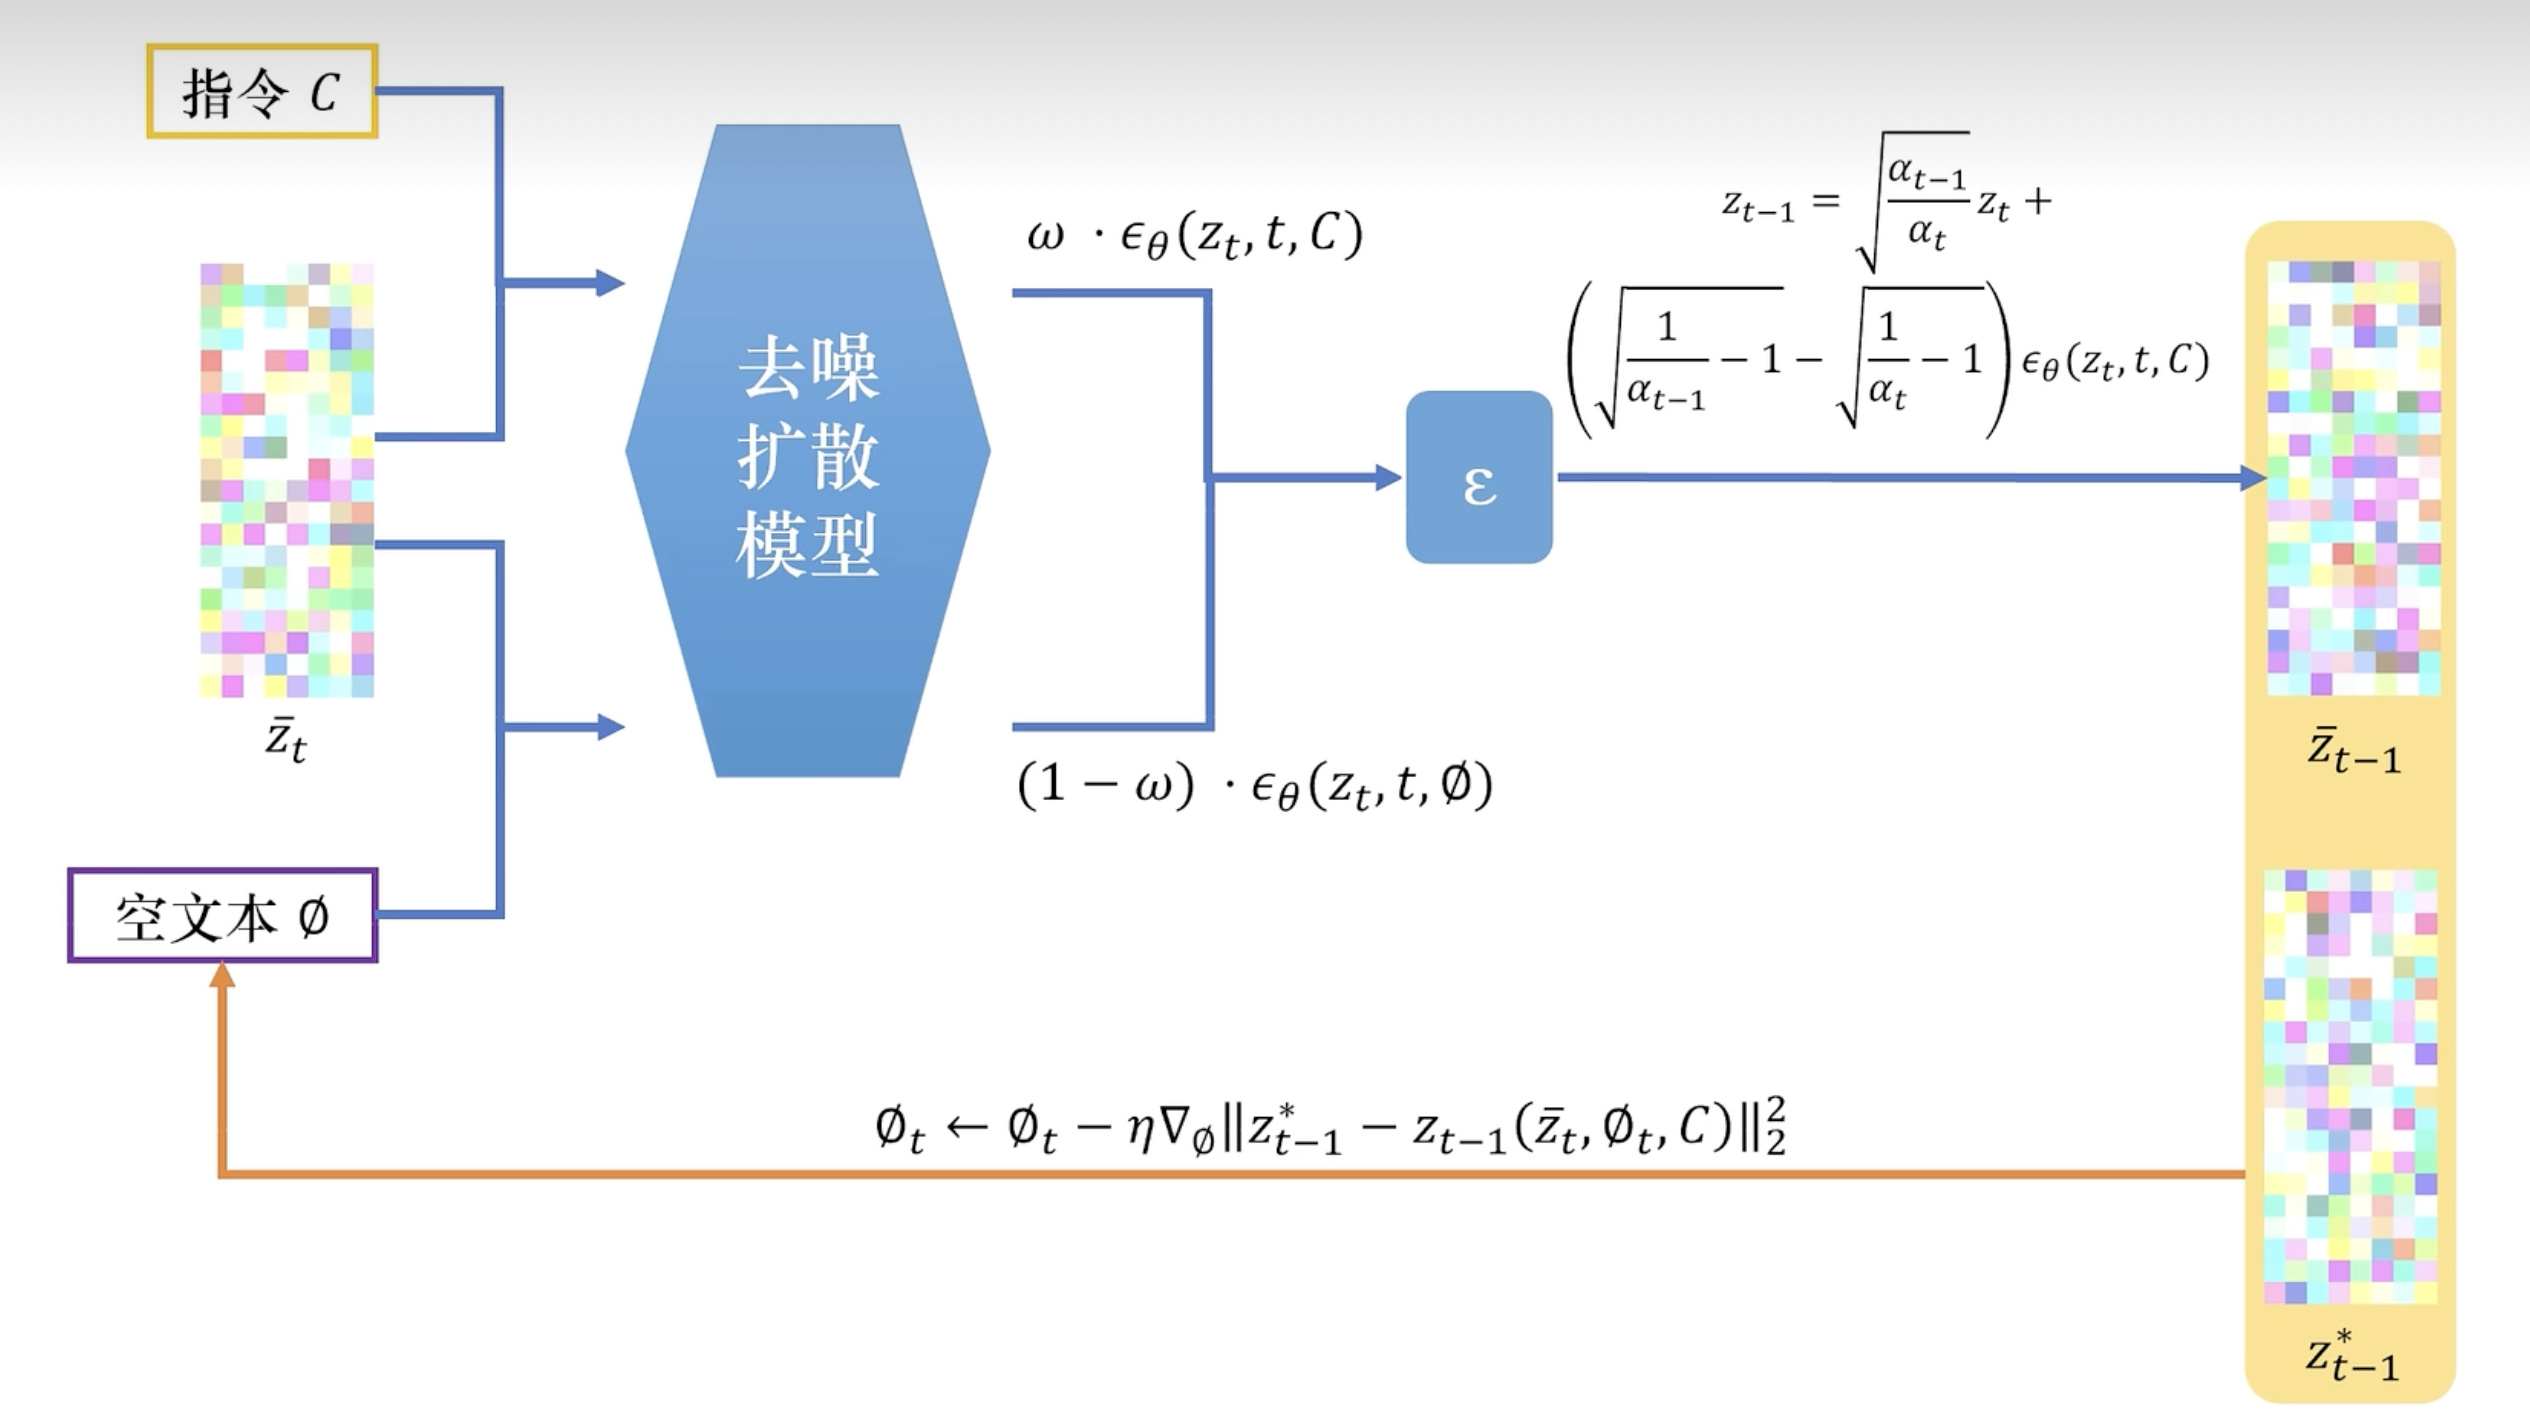
\includegraphics[width=0.95\textwidth]{images/image4.png}
    \caption{Classifier-Free Guidance 下的 DDIM Inversion 优化流程：模型同时输入隐变量 $\bar{z}_t$、目标指令 $C$ 与空文本 $\varnothing$，通过权重 $\omega$ 加权融合不同条件下的噪声预测结果，结合 DDIM 递推公式得到反向隐变量 $\bar{z}_{t-1}$；同时利用梯度公式迭代优化空文本特征，求解出优化后的隐变量 $z^*_{t-1}$，有效提升隐编码与原图、提示词的匹配度，为后续精细化图像编辑提供稳定可靠的隐空间基础。}
    \label{fig:ddim_cfg}
\end{figure}

\subsection{为什么大 $w$ 会导致重建失败？}

这个问题很关键，值得深入理解。

CFG 中的外推操作（式~\ref{eq:cfg_noise}）在采样时是好事——它让模型更加"听从"文本条件的指引。但在 Inversion 时，DDIM 的递推公式假设 $\epsilon_\theta(x_t, t)$ 是真正的 posterior mean 的某种估计。CFG 的外推\textbf{不是可逆的}——我们没法从 $\tilde{\epsilon}_\theta$ 精确反推出原始的 $\epsilon_\theta$。

具体来说：
\begin{enumerate}
    \item Inversion 时，我们用的是 CFG 噪声 $\tilde{\epsilon}_\theta$ 而不是原始噪声 $\epsilon_\theta$
    \item 采样时，我们也用 $\tilde{\epsilon}_\theta$
    \item 但由于 Inversion 的递推含有近似（$\epsilon_\theta(x_t, t) \approx \epsilon_\theta(x_{t-1}, t)$），CFG 放大了这个近似误差
    \item $w$ 越大，外推越远，误差越大，重建越差
\end{enumerate}

\textbf{解决方案：}一种常见的做法是在 Inversion 时使用较小的 $w$（甚至 $w=1$，即不用 CFG），在编辑/采样时再恢复到正常的 $w$。但这会引入 domain gap——Inversion 时的模型行为和采样时不一致。

更高级的方法（如 Null-text Inversion）会在 Inversion 过程中同时\textbf{优化空文本 embedding $\varnothing$}，来补偿 CFG 引入的偏差：

\begin{equation}\label{eq:null_text_opt}
    \varnothing^*_t = \arg\min_{\varnothing_t} \big\| x_{t-1}^{\text{target}} - \text{DDIM-Step}(x_t, \tilde{\epsilon}_\theta(x_t, t, C, \varnothing_t)) \big\|_2^2
\end{equation}

其中 $\varnothing_t$ 是每一步独立优化的空文本 embedding（原本所有步共享同一个空文本 embedding）。

\subsection{算法流程}

\begin{algorithm}[ht]
\caption{DDIM Inversion (with CFG)}
\label{alg:ddim_inversion}
\begin{algorithmic}[1]
\Require 真实图像 $x_0$，文本 prompt $C$，guidance scale $w$，总步数 $T$
\Ensure 反演 noise code $z_T$
\State $x \leftarrow x_0$
\For{$t = 1, \dots, T$}
    \State $\epsilon_{\text{cond}} \leftarrow \epsilon_\theta(x, t, C)$
    \State $\epsilon_{\text{uncond}} \leftarrow \epsilon_\theta(x, t, \varnothing)$
    \State $\tilde{\epsilon} \leftarrow \epsilon_{\text{uncond}} + w \cdot (\epsilon_{\text{cond}} - \epsilon_{\text{uncond}})$
    \State 用 $\tilde{\epsilon}$ 和 DDIM Inversion 公式从 $x$ 计算 $x_{\text{next}}$
    \State $x \leftarrow x_{\text{next}}$
\EndFor
\State \Return $z_T = x$
\end{algorithmic}
\end{algorithm}

\subsection{DDIM Inversion 的局限性}

\begin{enumerate}
    \item \textbf{近似误差累积：}每一步的 $\epsilon_\theta(x_t, t) \approx \epsilon_\theta(x_{t-1}, t)$ 近似会随着步数累积，导致 $T$ 较大时重建质量下降。
    \item \textbf{CFG 不兼容：}如前面讨论的，CFG 的外推操作与 Inversion 的可逆性假设冲突。
    \item \textbf{步数限制：}为了减小近似误差，通常需要跑满 $T$ 步（如 50-1000 步），不能像采样时那样大幅减少步子。
\end{enumerate}


% ═══════════════════════════════════════════════════════════════════════
%  5.  COMPARISONS & CONNECTIONS
% ═══════════════════════════════════════════════════════════════════════
\section{三种方法的比较与联系}

\subsection{方法对比总结}

\begin{center}
\begin{tabular}{c|c|c|c}
    \toprule
    \textbf{维度} & \textbf{Prompt-to-Prompt} & \textbf{Pivotal Inversion} & \textbf{DDIM Inversion} \\
    \midrule
    核心机制 & Attention 替换/重加权 & 直接优化 latent code & ODE 逆向递推 \\
    是否需要 inversion & 是（DDIM Inversion） & 否（自身就是 inversion） & 是 \\
    编辑粒度 & token/区域级别 & latent 级别 & latent 级别 \\
    重建质量 & 依赖 inversion 质量 & 高（直接优化） & 中等（近似误差） \\
    计算开销 & 低（仅 inference） & 高（需要优化） & 低（仅 inference） \\
    可控性 & 精细（逐 token 控制） & 中等 & 有限 \\
    \bottomrule
\end{tabular}
\end{center}

\subsection{三者的关系}

有趣的是，这三种方法并不是互相排斥的，而是可以\textbf{组合使用}：

\begin{enumerate}
    \item \textbf{DDIM Inversion + Prompt-to-Prompt：}先用 DDIM Inversion 将真实图像反演到 latent space，然后在去噪过程中使用 Prompt-to-Prompt 的 attention 编辑技术。这是最常见的组合方式，也是原 Prompt-to-Prompt 论文的做法。

    \item \textbf{Pivotal Inversion + Prompt-to-Prompt：}先用 Pivotal Inversion 得到更精准的 $z^*$（比 DDIM Inversion 重建更好），再在去噪/生成过程中应用 Prompt-to-Prompt 编辑。重建精度更高，但总耗时也更长。

    \item \textbf{DDIM Inversion + Pivotal 微调：}先用 DDIM Inversion 快速得到一个近似的 $z_T$，再以它为初始值，用 Pivotal Inversion 做少量几步优化微调。兼顾速度和精度。
\end{enumerate}

\subsection{实际使用建议 (Practical Considerations)}

\begin{itemize}
    \item \textbf{如果只需要简单编辑（换颜色、加修饰词）：}Prompt-to-Prompt + DDIM Inversion 就够了，速度快，效果也不差。
    \item \textbf{如果需要精确重建后再编辑：}考虑 Pivotal Inversion 或 Null-text Inversion，重建质量更好。
    \item \textbf{如果编辑涉及复杂的结构变化（如改变姿态、替换大物体）：}Pivotal Inversion 配合 cross-attention 调控的效果通常更好，因为更精准的 latent code 给了模型更稳定的起点。
    \item \textbf{Guidance scale 的选择：}Inversion 时 $w=1$（纯无条件或纯条件），编辑/采样时 $w=7.5$（正常 CFG），这是一个常用的工程 trick。虽然不完美，但大多数情况下够用。
\end{itemize}


% ═══════════════════════════════════════════════════════════════════════
%  6.  BEYOND INVERSION: RELATED WORK
% ═══════════════════════════════════════════════════════════════════════
\section{Beyond Inversion: 相关进展}

\subsection{Null-text Inversion}

Null-text Inversion 是 DDIM Inversion 的一个重要改进。核心 idea：

\begin{itemize}
    \item 不仅优化 latent code $z_T$，同时优化\textbf{每一步的空文本 embedding $\varnothing_t$}
    \item 这样可以在使用正常 CFG（$w=7.5$）的同时，保持完美的重建
    \item 优化开销：每一步独立优化一个低维 embedding，比 Pivotal Inversion 的 full optimization 轻量得多
\end{itemize}

\subsection{Textual Inversion}

Textual Inversion 的思路完全不同——它不是反演图像，而是\textbf{反演概念}：

\begin{itemize}
    \item 给定 3-5 张包含某个特定对象/风格的图片
    \item 学习一个新的 token embedding $v_*$（如 \texttt{<my-cat>}）
    \item 这个 token 就能在生成时精确触发该对象/风格
\end{itemize}

这为"个性化生成"（personalization）打开了大门——你可以教会模型认识你的猫、你的包、你的画风，然后用自然语言来创作。

\subsection{Encoder-based Inversion}

与其用优化或递推来反演，不如直接训练一个 encoder 网络：

\begin{equation}\label{eq:encoder}
    z_T = E_\phi(x_0)
\end{equation}

$E_\phi$ 是一个神经网络（通常是轻量级的），输入真实图像 $x_0$，直接输出其 latent code $z_T$。训练时可以用重建损失来监督。优势是\textbf{一次前向就完成 inversion}，速度极快；劣势是需要额外训练且泛化能力有限。

\subsection{Consistency Models 与 Inversion}

Consistency Models 将扩散模型的采样压缩为一步或几步，自然地也有其 Inversion 对应。由于 Consistency Models 学习的是 PF-ODE 的解，其 Inversion 理论上更加干净（没有近似误差累积的问题），是当前活跃的研究方向。


% ═══════════════════════════════════════════════════════════════════════
%  7.  SUMMARY
% ═══════════════════════════════════════════════════════════════════════
\section{总结}

\subsection*{核心要点速查}

\begin{center}
\begin{tabular}{c|l}
    \toprule
    \textbf{方法} & \textbf{一句话总结} \\
    \midrule
    Prompt-to-Prompt & 修改 attention map = 修改图像对应区域 \\
    Pivotal Inversion & 直接优化 $z$，让 $G(z)$ 逼近原图 \\
    DDIM Inversion & 把 DDIM 采样公式倒过来，从原图走向噪声 \\
    Null-text Inversion & 不仅反演图像，还优化空文本 embedding \\
    Textual Inversion & 反演概念而非图像，学会新的 token \\
    \bottomrule
\end{tabular}
\end{center}

\subsection*{关键 Insight}

\textbf{Inversion 的本质是建立"真实图像 $\leftrightarrow$ latent space"的双向桥梁。}一旦这座桥建好了，整个 latent space 的操作工具箱（插值、算术、编辑、控制）就都可以用于真实图像了。

回到文章开头提到的 trade-off（重建精度 vs 可编辑性），目前的研究趋势可以概括为两个方向：

\begin{enumerate}
    \item \textbf{提高重建精度：}Pivotal Inversion、Null-text Inversion 等方法通过优化或校正来逼近完美重建。
    \item \textbf{保持可编辑性：}通过正则化、约束优化范围来确保 $z$ 停留在"可编辑"区域内。
\end{enumerate}

\textbf{最后一点想法：}Inversion 是整个扩散模型实用化的关键一环。没有 Inversion，扩散模型只是一个"随机图片生成器"——很有趣但不实用。有了 Inversion，扩散模型就变成了一个\textbf{通用图像编辑器}——你可以拿任何一张真实照片来做各种修改。这就是为什么 Inversion 如此重要。


% ═══════════════════════════════════════════════════════════════════════
%  REFERENCES
% ═══════════════════════════════════════════════════════════════════════
\begin{thebibliography}{99}

\bibitem{p2p}
A. Hertz, R. Mokady, J. Tenenbaum, K. Aberman, Y. Pritch, and D. Cohen-Or,
\textit{Prompt-to-Prompt Image Editing with Cross-Attention Control},
ICLR, 2023.

\bibitem{pivotal}
D. Roich, R. Mokady, A. H. Bermano, and D. Cohen-Or,
\textit{Pivotal Tuning for Latent-based Editing of Real Images},
ACM Transactions on Graphics (TOG), 2022.

\bibitem{ddim}
J. Song, C. Meng, and S. Ermon,
\textit{Denoising Diffusion Implicit Models},
ICLR, 2021.

\bibitem{null_text}
R. Mokady, A. Hertz, K. Aberman, Y. Pritch, and D. Cohen-Or,
\textit{Null-text Inversion for Editing Real Images using Guided Diffusion Models},
CVPR, 2023.

\bibitem{textual_inversion}
R. Gal, Y. Alaluf, Y. Atzmon, O. Patashnik, A. H. Bermano, G. Chechik, and D. Cohen-Or,
\textit{An Image is Worth One Word: Personalizing Text-to-Image Generation using Textual Inversion},
ICLR, 2023.

\bibitem{ddpm}
J. Ho, A. Jain, and P. Abbeel,
\textit{Denoising Diffusion Probabilistic Models},
NeurIPS, 2020.

\bibitem{sde}
Y. Song, J. Sohl-Dickstein, D. P. Kingma, A. Kumar, S. Ermon, and B. Poole,
\textit{Score-Based Generative Modeling through Stochastic Differential Equations},
ICLR, 2021.

\end{thebibliography}

\end{document}
